\documentclass[11pt,a4paper]{article}

\usepackage{fontspec}
\setmainfont{DejaVu Sans}
\setmonofont{DejaVu Sans Mono}[Scale=0.82]
\usepackage[margin=1.8cm,top=1.65cm,bottom=1.7cm]{geometry}
\usepackage{xcolor}
\usepackage{tabularx}
\usepackage{booktabs}
\usepackage{array}
\usepackage{enumitem}
\usepackage{fancyhdr}
\usepackage{fancyvrb}
\usepackage{tikz}
\usetikzlibrary{arrows.meta,positioning,shapes.geometric,fit}
\usepackage{titlesec}
\usepackage{hyperref}

\definecolor{navy}{HTML}{173B57}
\definecolor{blue}{HTML}{1976A3}
\definecolor{lightblue}{HTML}{EAF4F8}
\definecolor{orange}{HTML}{D66B28}
\definecolor{lightorange}{HTML}{FFF0E4}
\definecolor{green}{HTML}{2E7D5B}
\definecolor{lightgreen}{HTML}{E8F5EE}
\definecolor{red}{HTML}{A33C35}
\definecolor{graytext}{HTML}{4A5560}
\definecolor{linegray}{HTML}{BCC7CE}

\hypersetup{colorlinks=true,linkcolor=navy,urlcolor=blue}
\setlength{\parindent}{0pt}
\setlength{\parskip}{5pt}
\setlist[itemize]{leftmargin=1.3em,itemsep=2pt,topsep=3pt}
\setlist[enumerate]{leftmargin=1.5em,itemsep=3pt,topsep=3pt}
\titleformat{\section}{\Large\bfseries\color{navy}}{\thesection.}{0.5em}{}
\titleformat{\subsection}{\large\bfseries\color{blue}}{}{0pt}{}

\pagestyle{fancy}
\fancyhf{}
\lhead{\small\color{graytext}Desarrollo de Aplicaciones II · Clase 9}
\rhead{\small\color{graytext}GOMARKET · Servicios Web}
\cfoot{\small\color{graytext}\thepage}
\renewcommand{\headrulewidth}{0.3pt}

\newcommand{\decisionbox}[1]{%
  \noindent\colorbox{lightorange}{\parbox{0.96\linewidth}{%
    \textbf{\color{orange}Decisión del equipo.} #1}}
}

\newcommand{\resultbox}[1]{%
  \noindent\colorbox{lightgreen}{\parbox{0.96\linewidth}{%
    \textbf{\color{green}Resultado.} #1}}
}

\begin{document}

\thispagestyle{empty}
\vspace*{1.1cm}
\begin{center}
  {\color{navy}\Huge\bfseries Actividad integradora}\par
  \vspace{4pt}
  {\color{blue}\LARGE Servicios Web: SOAP + mensajería}\par
  \vspace{12pt}
  {\Large GOMARKET · E-commerce}\par
  \vspace{20pt}
\end{center}

\decisionbox{Nuestro sistema, tal como está pensado hoy, \textbf{no necesita
SOAP}: sus componentes son propios y las integraciones modernas se resolverían
con REST y JMS. Para cumplir la actividad, diseñamos el caso hipotético indicado
por el profesor: \emph{si GOMARKET tuviera que conectarse con el ERP legado de un
proveedor, usaría SOAP para validar y reservar stock antes de aceptar la compra}.}

\vspace{16pt}
\begin{center}
\begin{tabularx}{0.88\linewidth}{>{\bfseries\color{navy}}p{4.2cm} X}
Materia & Desarrollo de Aplicaciones II \\
Tema & Integración sincrónica, SOAP, WSDL, JAX-WS y JMS \\
Equipo & Rodrigo, Nicolás, Tomás, Iván y Fol \\
Fecha & 2 de octubre de 2026 \\
Fuente & Clase 09, Unidad VI: Servicios Web \\
\end{tabularx}
\end{center}

\vfill
\begin{center}
\color{graytext}
\textbf{Entregable solicitado}\par
Diagrama de integración · contrato SOAP · mensajería · justificación y fallas
\end{center}

\newpage
\section{Escenario elegido}

Una persona confirma el carrito. GOMARKET necesita saber si el proveedor puede
reservar las unidades antes de aceptar el pedido. En el sistema real actual esa
consulta no existe; el catálogo y el stock pertenecen a la propia aplicación.

Para el ejercicio suponemos que parte del stock está administrado por un
\textbf{ERP legado externo} que sólo ofrece un servicio SOAP. El flujo es:

\begin{enumerate}
  \item GOMARKET llama de manera \textbf{sincrónica} al ERP para validar y reservar stock.
  \item Si el ERP acepta, GOMARKET encola el pedido para procesarlo sin bloquear al usuario.
  \item Cuando el pedido queda confirmado, publica un evento para notificación,
        auditoría y estadísticas.
\end{enumerate}

\section{Diagrama de integración}

\begin{center}
\resizebox{\textwidth}{!}{%
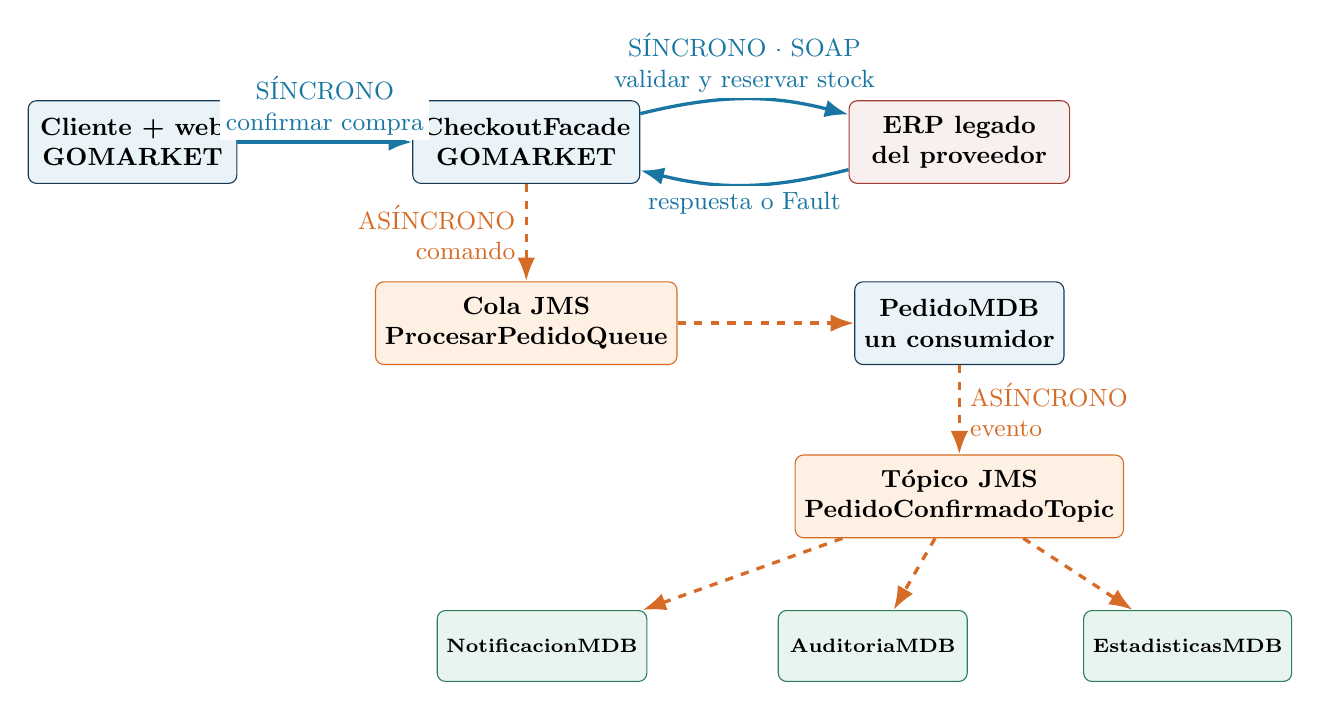
\begin{tikzpicture}[
  box/.style={draw=navy,rounded corners=3pt,fill=lightblue,minimum width=2.65cm,minimum height=1.05cm,align=center,font=\small\bfseries},
  external/.style={draw=red,rounded corners=3pt,fill=red!8,minimum width=2.8cm,minimum height=1.05cm,align=center,font=\small\bfseries},
  broker/.style={draw=orange,rounded corners=3pt,fill=lightorange,minimum width=2.8cm,minimum height=1.05cm,align=center,font=\small\bfseries},
  consumer/.style={draw=green,rounded corners=3pt,fill=lightgreen,minimum width=2.4cm,minimum height=.9cm,align=center,font=\scriptsize\bfseries},
  sync/.style={-{Latex[length=3mm]},very thick,blue},
  async/.style={-{Latex[length=3mm]},very thick,dashed,orange},
  every node/.style={font=\small}
]
\node[box] (web) at (0,0) {Cliente + web\\GOMARKET};
\node[box] (checkout) at (5.0,0) {CheckoutFacade\\GOMARKET};
\node[external] (erp) at (10.5,0) {ERP legado\\del proveedor};
\node[broker] (queue) at (5.0,-2.3) {Cola JMS\\ProcesarPedidoQueue};
\node[box] (pedido) at (10.5,-2.3) {PedidoMDB\\un consumidor};
\node[broker] (topic) at (10.5,-4.5) {Tópico JMS\\PedidoConfirmadoTopic};
\node[consumer] (notif) at (5.2,-6.4) {NotificacionMDB};
\node[consumer] (audit) at (9.4,-6.4) {AuditoriaMDB};
\node[consumer] (stats) at (13.4,-6.4) {EstadisticasMDB};

\draw[sync] (web) -- node[above,fill=white,inner sep=2pt,align=center]{SÍNCRONO\\confirmar compra} (checkout);
\draw[sync] (checkout) to[bend left=14] node[above,fill=white,inner sep=2pt,align=center]{SÍNCRONO · SOAP\\validar y reservar stock} (erp);
\draw[sync] (erp) to[bend left=14] node[below,fill=white,inner sep=2pt,align=center]{respuesta o Fault} (checkout);
\draw[async] (checkout) -- node[left,align=right]{ASÍNCRONO\\comando} (queue);
\draw[async] (queue) -- (pedido);
\draw[async] (pedido) -- node[right,align=left]{ASÍNCRONO\\evento} (topic);
\draw[async] (topic) -- (notif);
\draw[async] (topic) -- (audit);
\draw[async] (topic) -- (stats);
\end{tikzpicture}}
\end{center}

\begin{tabularx}{\textwidth}{@{}>{\bfseries\color{blue}}p{3.2cm} X@{}}
Flecha azul continua & Interacción sincrónica: el emisor espera la respuesta. \\
Flecha naranja punteada & Interacción asincrónica: el broker conserva y entrega el mensaje. \\
\end{tabularx}

\newpage
\section{Contrato del servicio SOAP}

\subsection{Operación propuesta}

\begin{tabularx}{\textwidth}{@{}>{\bfseries\color{navy}}p{3.5cm} X@{}}
Servicio & \texttt{InventarioLegadoService} \\
Operación & \texttt{validarYReservarStock} \\
Entrada & \texttt{idSolicitud}, \texttt{idPedido} y lista de ítems con producto y cantidad \\
Respuesta & \texttt{idReserva}, estado, vencimiento y detalle de unidades reservadas \\
Faults & \texttt{StockInsuficienteFault}, \texttt{ProductoInexistenteFault} y fallo técnico del proveedor \\
Estilo & SOAP 1.2, document/literal wrapped \\
\end{tabularx}

La variante \emph{document/literal wrapped} permite validar el Body contra un
XSD y es la alternativa recomendada en la clase para interoperabilidad.

\subsection{Interfaz Java anotada con JAX-WS}

\begin{Verbatim}[frame=single,framesep=7pt,rulecolor=\color{linegray},fontsize=\small]
import jakarta.jws.WebMethod;
import jakarta.jws.WebParam;
import jakarta.jws.WebResult;
import jakarta.jws.WebService;
import jakarta.jws.soap.SOAPBinding;

@WebService(
  name = "InventarioLegadoPort",
  targetNamespace = "https://proveedor.example/inventario")
@SOAPBinding(
  style = SOAPBinding.Style.DOCUMENT,
  use = SOAPBinding.Use.LITERAL,
  parameterStyle = SOAPBinding.ParameterStyle.WRAPPED)
public interface InventarioLegadoPort {

  @WebMethod(operationName = "validarYReservarStock")
  @WebResult(name = "resultadoReserva")
  ResultadoReserva validarYReservarStock(
      @WebParam(name = "solicitud") SolicitudReserva solicitud)
      throws StockInsuficienteFault, ProductoInexistenteFault;
}
\end{Verbatim}

El WSDL generado describe los tipos, mensajes, \texttt{portType}, binding SOAP y
endpoint. El cliente de GOMARKET genera su proxy desde ese contrato; no depende
del código interno del ERP.

\newpage
\subsection{Fault de negocio requerido}

\begin{Verbatim}[frame=single,framesep=7pt,rulecolor=\color{linegray},fontsize=\small]
<soap:Fault>
  <soap:Code><soap:Value>soap:Sender</soap:Value></soap:Code>
  <soap:Reason>
    <soap:Text xml:lang="es">Stock insuficiente</soap:Text>
  </soap:Reason>
  <soap:Detail>
    <inv:stockInsuficiente codigo="STOCK-409">
      <producto>PROD-25</producto>
      <solicitado>3</solicitado>
      <disponible>1</disponible>
    </inv:stockInsuficiente>
  </soap:Detail>
</soap:Fault>
\end{Verbatim}

Este Fault es una respuesta funcional: el pedido fue entendido, pero no se puede
reservar la cantidad solicitada. GOMARKET informa el problema y no encola el pedido.

\section{Mensajería}

\small
\begin{tabularx}{\textwidth}{@{}>{\raggedright\arraybackslash}p{2.95cm} >{\raggedright\arraybackslash}p{3.2cm} >{\raggedright\arraybackslash}p{2.8cm} X@{}}
\toprule
\textbf{Mensaje} & \textbf{Destino} & \textbf{Consumidores} & \textbf{Por qué} \\
\midrule
\texttt{ProcesarPedido} & Cola\par{\scriptsize\texttt{ProcesarPedidoQueue}} & \texttt{PedidoMDB} & Es una orden que debe procesarse exactamente una vez por un consumidor. La cola amortigua picos y conserva el mensaje si el consumidor está caído. \\
\addlinespace
\texttt{PedidoConfirmado} & Tópico\par{\scriptsize\texttt{PedidoConfirmadoTopic}} & Notificación, Auditoría y Estadísticas & Es un hecho que interesa a varios componentes. Cada suscriptor recibe su propia copia sin acoplar al productor. \\
\addlinespace
\texttt{ReintentarReserva} & Cola\par{\scriptsize\texttt{ReintentarReservaQueue}} & \texttt{ReservaStockMDB} & Sólo se usa cuando el ERP no responde. Permite reintentar fuera de la petición del usuario. \\
\bottomrule
\end{tabularx}
\normalsize

\subsection{Contenido mínimo de los mensajes}

Se utilizaría \texttt{TextMessage} con JSON para no compartir clases Java entre
productor y consumidores. Todos los mensajes llevan:

\begin{itemize}
  \item \texttt{idEvento} e \texttt{idPedido} para trazabilidad e idempotencia;
  \item \texttt{tipoEvento}, \texttt{version} y \texttt{fecha};
  \item los datos mínimos necesarios; nunca contraseñas ni datos de pago completos.
\end{itemize}

\begin{Verbatim}[frame=single,framesep=4pt,rulecolor=\color{linegray},fontsize=\scriptsize]
{
  "idEvento": "EVT-7f41",
  "tipoEvento": "PedidoConfirmado",
  "version": 1,
  "fecha": "2026-10-02T12:30:00-03:00",
  "idPedido": "PED-1042",
  "idReserva": "RES-8831",
  "total": 92000.00
}
\end{Verbatim}

\section{Justificación de cada tramo}

\begin{tabularx}{\textwidth}{@{}>{\bfseries}p{3.5cm} p{2.3cm} X@{}}
\toprule
Tramo & Elección & Justificación \\
\midrule
GOMARKET → ERP legado & Sincrónico SOAP & La compra no puede avanzar sin saber si el stock quedó reservado. El usuario espera una respuesta concreta en pantalla y el ERP sólo ofrece contrato WSDL/SOAP. \\
GOMARKET → procesamiento & Asincrónico, cola & Una vez reservado el stock, el trabajo puede continuar después. La cola desacopla tiempos, amortigua carga y entrega la orden a un único procesador. \\
Pedido → interesados & Asincrónico, tópico & Notificar, auditar y actualizar estadísticas no debe demorar la compra. Hay varios interesados independientes en el mismo evento. \\
\bottomrule
\end{tabularx}

\section{Fallas y timeout de 5 segundos}

Un timeout no significa que el ERP no haya reservado; significa que GOMARKET no
recibió la respuesta a tiempo. Repetir sin control podría reservar dos veces.

\begin{enumerate}
  \item La llamada SOAP usa un timeout de conexión y lectura de \textbf{5 segundos}.
  \item Cada intento envía el mismo \texttt{idSolicitud}. El ERP debe tratarlo como
        clave idempotente: repetirlo devuelve la reserva existente, no crea otra.
  \item Si no hay respuesta, GOMARKET \textbf{no confirma ni cobra} la compra. El
        pedido queda \texttt{PENDIENTE\_VALIDACION} y la pantalla informa:
        ``Estamos verificando el stock; te avisaremos el resultado''.
  \item Se publica \texttt{ReintentarReserva} en una cola. Se hacen dos reintentos
        con espera creciente (2 y 4 segundos), fuera de la petición web.
  \item Si vuelve a fallar, el mensaje pasa a \texttt{ReservaStockDLQ}; se registra
        la correlación y se alerta para revisión. No se pierde silenciosamente.
  \item Si el ERP responde con \texttt{StockInsuficienteFault}, el pedido se marca
        rechazado y se informa al cliente. Si responde correctamente, el flujo
        continúa por \texttt{ProcesarPedidoQueue}.
\end{enumerate}

Después de varios fallos consecutivos se abre un \emph{circuit breaker} por un
tiempo corto para no saturar al ERP. Esta medida complementa al timeout: evita
fallas en cadena, una debilidad propia de la integración sincrónica.

\subsection{Diferencia entre errores}

\small
\begin{tabularx}{\textwidth}{@{}>{\bfseries\raggedright\arraybackslash}p{4.5cm} X X@{}}
\toprule
Caso & Qué significa & Acción de GOMARKET \\
\midrule
Stock insuficiente\\{\scriptsize\texttt{StockInsuficienteFault}} & El ERP respondió y rechazó por una regla de negocio. & Rechazar el pedido, informar disponibilidad y permitir editar el carrito. \\
Producto inexistente\\{\scriptsize\texttt{ProductoInexistenteFault}} & El código enviado no existe en el legado. & No reintentar; registrar inconsistencia de catálogo. \\
Timeout / red caída & No sabemos si el ERP procesó el pedido. & Estado pendiente, reintento idempotente y eventual DLQ. \\
\texttt{soap:Receiver} & Falló el servidor del proveedor. & Reintentar con límite; abrir circuito si persiste. \\
\bottomrule
\end{tabularx}
\normalsize

\section{Conclusión}

\resultbox{GOMARKET no incorpora SOAP por capricho ni porque sus componentes
internos lo requieran. En este escenario hipotético se usaría únicamente para
interoperar con un proveedor legado que publica un WSDL. La validación de stock
es sincrónica porque condiciona la compra; el procesamiento, las notificaciones,
la auditoría y las estadísticas son asincrónicos porque pueden ocurrir después y
se benefician del desacople de JMS.}

\vfill
{\small\color{graytext}
Contenido elaborado a partir de las 44 diapositivas de
\emph{Clase09\_UnidadVI\_ServiciosWeb}: integración sincrónica, SOAP 1.2, WSDL,
JAX-WS, mensajería y actividad final (diapositivas 41--44).}

\end{document}
